% Using KOMA Script document style
% Font size setting and
% option to skip empty lines as new paragraphs
\documentclass[10pt,a4paper]{article}
% Packages without Options
\usepackage{
	algorithm,
	alltt,
	algpseudocode,
	amsfonts,
	amssymb,
	appendix,
	array,
	booktabs,
	dirtree,
	enumitem,
	float,
	footnote,
	gensymb,
	geometry,
	graphicx,
	interval,
	karnaugh-map,
	lipsum,
	listings,
	longtable,
	makecell,
	mathtools,
	minted,
  nicematrix,
	parskip,
	pdfpages,
	pgfkeys,
	pgfplots,
	subcaption,
	tabularx,
	tablefootnote,
	textcomp,
	tikz,
    titlecaps,
	venndiagram,
	wrapfig,
	wrapfig,
	xcolor
}



% Packages with Options

\usepackage[framemethod=tikz]{mdframed}
\usepackage[colorlinks,linkcolor=cyan, citecolor=cyan, urlcolor=cyan]{hyperref}
\usepackage[labelfont=bf,textfont=it,labelsep=period]{caption}
\usepackage[RPvoltages]{circuitikz}
\usepackage[english]{babel}
\usepackage[nameinlink,noabbrev]{cleveref}

\definecolor{mintedbackground}{rgb}{0.97,0.97,0.97}

\setminted[cpp]{
bgcolor=mintedbackground,
    linenos=true,
    breaklines=true,}

\setminted[js]{
bgcolor=mintedbackground,
    linenos=true,
    breaklines=true,}

\setminted[python]{
bgcolor=mintedbackground,
    linenos=true,
    breaklines=true,}
    

\linespread{1.5}

% Package: AlgorithmicX
% Sets all comments to be indentend and aligned

\renewcommand{\Comment}[2][.7\linewidth]{%
  \leavevmode\hfill\makebox[#1][l]{//~#2}}


% Package: Interval
% Sets the style of mathematical intervals
\intervalconfig{
soft open fences, separator symbol=,,
}

% Package: Geometry
% Sets the page margins
\geometry{
    a4paper,
    left=32mm,
    right=22mm,
    top=22mm,
    }
	
% Creates a proper caption name for algorithms
\newcommand{\algorithmautorefname}{Algorithm}
\newcommand{\listingautorefname}{Listing}
\algrenewcommand{\algorithmiccomment}[1]{\texttt{// #1} }
% Creates a numbered environment for Theorems
\newtheorem{theorem}{Theorem}

% Redefine the implication arrow to be a simple, thin arrow instead of the default, thick arrow
\renewcommand{\implies}{\rightarrow}

% Create a new command for the set complement to make my logical statements easier to read
\newcommand{\compl}{\overline}

% Creates commands for combinatorics nCr and nPr
\newcommand{\nCr}[2]{\,_{#1}C_{#2}} % nCr
\newcommand{\nPr}[2]{\,_{#1}P_{#2}} % nPr

% Package: tikz
% Loads libraries for drawing automata, 
\usetikzlibrary{automata,positioning,shadows,arrows, shapes.gates.logic.US, calc}

% Creates a command to create a button shape
\newcommand*\keystroke[1]{%
  \tikz[baseline= (key.base)]
    \node[%
      draw,
      fill=white,
      drop shadow={shadow xshift=0.25ex,shadow yshift=-0.25ex,fill=black,opacity=0.75},
      rectangle,
      rounded corners=2pt,
      inner sep=1pt,
      line width=0.5pt,
      font=\scriptsize\sffamily
    ] (key) {#1\strut};
}

% Package: pgfplot
% Sets the global options for PGF Plots
\pgfplotsset{compat=newest}

% Package: tikz
% Flowchart Shapes
\tikzstyle{startstop} = [rectangle, rounded corners, minimum width=3cm, minimum height=1cm,text centered, draw=black, fill=red!30]
\tikzstyle{io} = [trapezium, trapezium left angle=70, trapezium right angle=110, minimum width=3cm, minimum height=1cm, text centered, draw=black, fill=blue!30]
\tikzstyle{process} = [rectangle, minimum width=3cm, minimum height=1cm, text centered, draw=black, fill=orange!30]
\tikzstyle{decision} = [diamond, minimum width=3cm, minimum height=1cm, text centered, draw=black, fill=green!30]
\tikzstyle{arrow} = [thick,->,>=stealth]

% Disable Minted syntax error highlights (red boxes)
\AtBeginEnvironment{minted}{%
  \renewcommand{\fcolorbox}[4][]{#4}}

% Listings Style (non-minted)

\lstdefinestyle{arjuncode}{
    basicstyle=\ttfamily,
    breakatwhitespace=false,         
    breaklines=true,                 
    captionpos=b,                    
    keepspaces=true,                 
    numbers=left,                    
    numbersep=5pt,                  
    showspaces=false,                
    showstringspaces=false,
    showtabs=false,                  
    tabsize=2
}

\lstset{style=arjuncode}

\graphicspath{{images/}}


\title{CM1020: Discrete Mathematics \\ Peer-Graded Assignment 2.109}
\author{Arjun Muralidharan}
\begin{document}
\maketitle
\pagebreak
\newpage
\renewcommand{\subsubsectionautorefname}{section\negthinspace}
% Preamble: 
\section*{Question 1}

We can show a function \( A \rightarrow B \)  to be injective by showing that if \( f(x_1) = f(x_2) \) for arbtirary \( x_1, x_2 \in A \), then \( x_1 = x_2 \). We can disprove it by showing that more than one function value is possible for a given element.

We can show a function \( A \rightarrow B \) to be surjective by showing that for an arbitrary element \( y \in B \) there is an element \( x \in A \) such that \( f(x) = y \). We can disprove it by finding an element that does not have a function value.

\paragraph{Function 1} To show that the function \[
f_1: \mathbb{R} \rightarrow \mathbb{R} \text{ where } f(x) = x^2 + 1  
\]
is injective, we see if \( f(x) = f(y) \) for arbtirary \( x_1, x_2 \in A \), then \( x = y \).

\begin{align}
  {x_1}^2 + 1 &= {x_2}^2 + 1 \\
  {x_1}^2 &= {x_2}^2 \\
  \pm x_1 &= \pm x_2
\end{align}

Therefore \( x_1 \neq x_2 \) and the function is \textbf{not injective}. For example: \( x_1 = -2, x_2 = 2 \) and \( f(x_1) = f(x_2) = 4 \). The function is \textbf{not surjective} as there exist elements in the co-domain that do not have a function value \( f(x) \), for example \( f(x) = -2 \).    

\paragraph{Function 2} The function \[
  f_2: \mathbb{R} \rightarrow \interval[open right]{-1}{\infty} \text{ where } f(x) = x^2 + 1
  \]
is \textbf{not injective} as per the reasoning for function \( f_1 \). 
As the co-domain is restricted to positive real numbers, The function is \textbf{surjective} as there exist pre-images \( x \) for any \( f(x) \).

\paragraph{Function 3} The function 
\[
  f_2: \mathbb{R} \rightarrow \mathbb{R} \text{ where } f(x) = x^3
\]

can be shown to be \textbf{injective} as it is a \textbf{strictly increasing} and \textbf{real-valued} function. Therefore for any given \( x_1, x_2 \) we know that \( f(x_1) \neq f(x_2) \). The plot for this function is shown in \autoref{plots1}. The function is \textbf{surjective} as \( f(x) \) is defined for any \( x \).

\paragraph{Function 4} The function \[
  f_2: \mathbb{R} \rightarrow \interval[open right]{-1}{\infty} \text{ where } f(x) = 2x + 3
\]

is \textbf{injective} because it is a \textbf{strictly increasing} and \textbf{real-valued} function. For each \( x \) there is a unique \( f(x) \) in the co-domain. The function is \textbf{surjective} as \( f(x) \) is defined for any \( x \).

\paragraph{Function 5} The function \[
  f_2: \mathbb{Z} \rightarrow \mathbb{Z} \text{ where } f(x) = 2x + 3
\]

is \textbf{injective} because it is a \textbf{strictly increasing} and \textbf{integer-valued} function. For each \( x \) there is a unique \( f(x) \) in the co-domain. The function is \textbf{not surjective} as \( f(x) \) is not defined for any \( x \), for example \( f(1) \) is not defined in the co-domain \( \mathbb{Z} \). 

\begin{figure}[h]
  \centering
  \caption{Plots for Question 1}\label{plots1}
  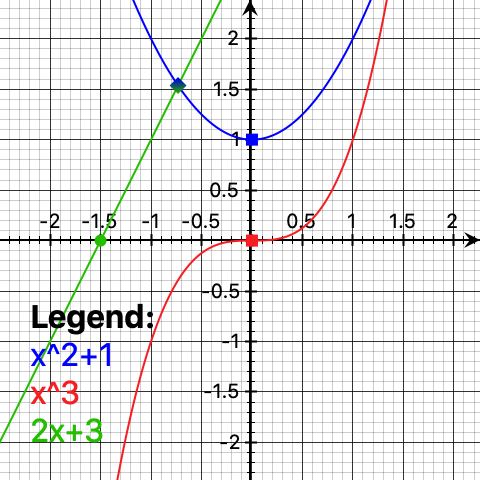
\includegraphics[]{plots.png}
\end{figure}

\section*{Question 2}
\begin{enumerate}
  \item The function \( f_2: \mathbb{R} \rightarrow \interval[open]{-1}{\infty} \text{ where } f(x) = e^x + 1 \) is a bijection if it is both injective and surjective. It is injective because it is \textbf{strictly increasing} and each \( x \in \mathbb{R} \) has a unique \( f(x) \in \mathbb{R} \).
  \item  The inverse of the function is given as follows: \begin{align}
    f^-1 = e^y + 1 &= x \\
    e^y &= x-1 \\
    \ln(e^y) &= \ln(x-1) \\
    y &= \ln(x-1)
  \end{align}

  \item The plots are given in \autoref{plots2}.
  \item The graphs are both strictly increasing. The graph of \( f \) is exponential growth, while the graph of \( f^-1 \) is logarithmic growth. The graphs are symmetric.
\end{enumerate} 

\begin{figure}[h]
  \centering
  \caption{Plots for Question 2}\label{plots2}
  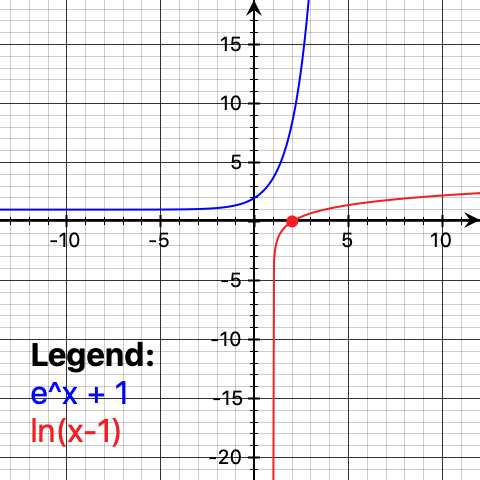
\includegraphics[]{expplot.png}
\end{figure}

\end{document}

